%% eval.tex
\chapter{Use-Case - Die Suche nach dem besten Auto}
\label{ch:useCase}
%% ==============================
Jeder hat beim Kauf eines Autos seine eigene Wünsche bzw. Kriterien. Viele wollen eine hohe PS Leistung, andere interessiert nur ein geringer Preis. Bei einem einzigen Kriterium (z.B. der Preis soll unter 16000 \euro liegen), kann es passieren, dass es zu viele Autos gibt, die dieses Kriterium erfüllen.
Im Gegensatz dazu gibt es für Kundenwünsche mit mehreren Kriterien oft gar keine entsprechenden Autos, da Kriterien als harte Bedingungen gewertet werden und somit alle erfüllt sein müssen. Diese beiden Situationen erschweren es einem Autoverkäufer ein passendes Auto für den Kunden anzubieten. Damit dieses Problem gelöst wird, werden zuerst die Kundenwünsche in Präferenzen umgewandelt. Präferenzen sorgen dafür, dass Kundenwünsche nicht perfekt erfüllt werden müssen, sondern nur so gut wie möglich. Anschließend wird mithilfe dieser Präferenzen eine Skyline und eine repräsentative Skyline für weitere Reduzierung der Ergebnismenge gebildet. Dadurch tauchen keine Autos mehr in der Ergebnismenge auf, die bezüglich der Präferenzen schlechter sind als andere.
Das Ziel dieses Kapitels ist es diese Vorgehensweise mit den implementierten KNIME Nodes an Beispieldaten zu veranschaulichen.
%% ==============================
\section{Datenvorbereitung}
\label{ch:Evaluierung:sec:vorbereitung}
%% ==============================
Zuerst müssen die Dimensionen, die für die Wünsche eines ausgedachten Kunden von Bedeutung sind, ausgewählt werden. Davor werden allerdings alle Dimensionen der vorliegenden Datensätze bzw. Autos vorgestellt. Die Dimensionen entsprechen den Spaltennamen der Autodaten und sind wie folgt benannt: id, name, make, color, price, age, horsepower, fuel, idowner, city\textunderscore consumption, mileage, description, reg\textunderscore date, highway\textunderscore consumption

Die Daten liegen in einer PostgreSQL Datenbank vor. Mittels des Database Connector wird eine Verbindung zu dieser Datenbank hergestellt. Damit eine erfolgreiche Datenbankverbindung aufgebaut werden kann, müssen im NodeDialog dieses Nodes wichtige Daten wie Datenbank URL, JDBC-Treiber, Username und Passwort eingegeben werden (siehe Abbildung \ref{img:nodeDialogConnector}). 

\begin{figure}[H]
	\centering
	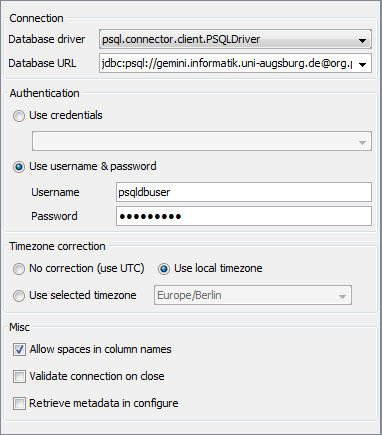
\includegraphics[width=0.6\textwidth]{nodeDialogConnector.png}
	\caption{NodeDialog des Database Connector Nodes}
	\label{img:nodeDialogConnector}
\end{figure} 

Der Node gibt eine Datenbankverbindung als Ausgabe zurück, die als Eingabe für den Database Table Selector und dem Database Reader Node dient. Diese beiden Nodes benötigen im NodeDialog einen SQL-Query als Eingabe. Für dieses Beispiel wird der Query \textit{SELECT * FROM car} eingegeben, da mit allen Autodatensätzen und allen Dimensionen weitergearbeitet werden soll. Es ist jedoch möglich die Datensätze hier schon mit einer \textit{WHERE} Klausel einzuschränken, falls dies gewünscht ist.

Die Ausgabe des Database Table Selector ist die Datenbankverbindung, die als Eingabe in den Node kommt und mit dem eingegebenen Query als Zusatzinformation zurückgegeben wird. Der Database Reader gibt im Gegensatz dazu einen BufferedDataTable aus. Dieser entsteht durch die Abfrage des eingegebenen SQL-Querys an die Datenbank und stellt die Daten aller Auto mit ihren Dimensionen in einer Tabelle dar. 

Hierbei muss beachtet werden, dass beide Nodes eine identische Datenbankverbindung und den selben Query im NodeDialog als Eingabe bekommen sollten. Falls dies nicht der Fall ist, liefert der PreferenceCreator Node, der sowohl die Datenbankverbindung mit dem Query als auch den BufferedDataTable als Eingabe bekommt, einen Fehler.

Nun da alle Vorbereitungen getroffen sind, können Präferenzen für die Kundenwünsche erstellt werden. Der bisherige Stand des KNIME Workflows ist in Abbildung \ref{img:datenVorbereitung} zu sehen.

\begin{figure}[H]
	\centering
	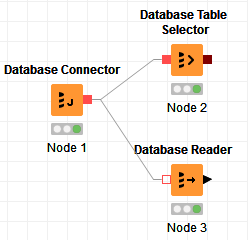
\includegraphics[width=0.6\textwidth]{datenVorbereitung.png}
	\caption{Workflow mit Database Connector, Database Table Selector und Database Reader Node}
	\label{img:datenVorbereitung}
\end{figure} 
%% ==============================
\section{Erstellung von Präferenzen}
\label{ch:Evaluierung:sec:createPref}
%% ==============================
Nun da die nötigen Eingaben für den PreferenceCreator vorhanden sind, können die Präferenzen für ausgewählte Dimensionen erstellt werden. Den BufferedDataTable benutzt dieser Node, um eine Auswahlbox für die Dimensionen und eine Auswahlbox für die Werte dieser Dimensionen zu erstellen. Die Datenbankverbindung wird für folgende Nodes benötigt, da diese mit den vom PreferenceCreator erstellten Score-Query eine Scoretabelle erstellen können und mit diesen Scores anstatt der eigentlichen Daten weiterarbeiten. 
Der für dieses Kapitel ausgedachte Kunde hat folgende Präferenzen: Er möchte ein Auto mit einem niedrigen Preis, einer hohen PS Leistung und einem niedrigen Kilometerstand. Darüber hinaus möchte er, dass das Auto nicht zu alt ist, was jedoch nicht so wichtig ist wie der Preis. Ebenfalls würde er ein grünes und schwarzes Auto vorziehen und auf keinen Fall ein rotes Auto wollen. Die Farbe ist jedoch nicht so wichtig wie die PS Leistung. Aus diesen Wünschen ergeben sich die Präferenzen in Abbildung \ref{img:useCaseNodeDialog}. Hier ist auch ein Button zu erkennen, der den Preference-Query für die aktuelle Nodebaumstruktur zeigt. So kann falls gewünscht zu jeder Zeit geprüft werden, ob die Nodebaumstruktur dem entspricht, was erreicht werden soll. 

\begin{figure}[H]
	\centering
	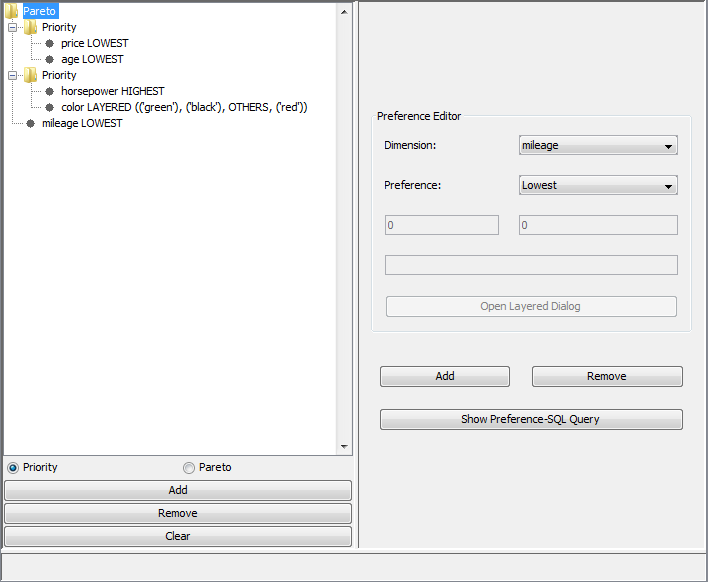
\includegraphics[width=0.6\textwidth]{useCaseNodeDialog.png}
	\caption{Präferenzen für den besten Basketballspieler}
	\label{img:useCaseNodeDialog}
\end{figure} 

Nach der Ausführung des Nodes wird die vorhandene Datenbankverbindung und Flowvariablen mit Preference- und Scorequery als Inhalt zurückgegeben. 

Der aktuelle Workflow ist in Abbildung \ref{img:preferenceWorkflow} zu sehen und wird im nächsten Abschnitt mit (repräsentativen) Skyline Nodes wie den DistanceBasedResolver erweitert. 

\begin{figure}[H]
	\centering
	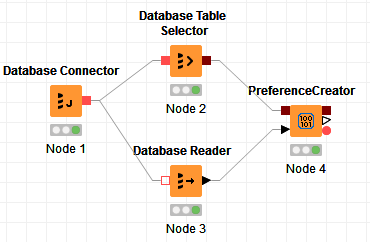
\includegraphics[width=0.6\textwidth]{preferenceWorkflow.png}
	\caption{Workflow mit dem PreferenceCreator Node}
	\label{img:preferenceWorkflow}
\end{figure}  
%% ==============================
\section{Reduzierung der Datensätze}
\label{ch:Evaluierung:sec:repSkyline}
%% ==============================
Wie erwähnt gibt der PreferenceCreator Node als Ausgabe eine Datenbankverbindung zurück. Mit dieser Verbindung kommen noch versteckte Flowvariablen in die nachfolgenden Nodes. Diese beinhalten Score-Query, Preference-Query und die in ein spezielles Format konvertierte Baumstruktur des NodeDialogs. Diese Datenbankverbindung und die Flowvariablen benutzt der Block-Nested-Loop, um eine Skyline zu erstellen. Im NodeDialog des Block-Nested-Loop Nodes wurde für das Fenster des Algorithmus ein Wert von vier eingegeben, da dieser Wert für die 300 original Datensätze  nicht zu groß und nicht zu klein ist. Nach Ausführung des Nodes wird eine Skyline mit 27 Datensätzen ausgegeben (siehe \ref{img:skyline}). Dadurch werden alle Datensätze die basierend auf den Präferenzen schlechter sind als andere für weitere Betrachtungen ausgeschlossen.

\begin{figure}[H]
	\centering
	
\includegraphics[width=0.6\textwidth]{skyline.png}
	\caption{Skyline des Autobeispiels}
	\label{img:skyline}
\end{figure} 

Mit dieser Anzahl von Skylinedatensätzen ist es jedoch immer noch schwer das beste Auto für den Kunden auszuwählen. Aus diesem Grund muss ergänzend die repräsentative Skyline bestimmt werden.

Den Anfang macht der DominationMaximizer. Für diesen Node muss im NodeDialog die Größe der repräsentativen Skyline eingegeben werden. Für das Beispiel in diesem Kapitel, wurde der Wert $k=4$ genommen. Es ergibt sich die repräsentative Skyline in Abbildung \ref{img:domMaximizer}. An den Werten der einzelnen Dimensionen ist zu erkennen, dass die Datensätze nah aneinander liegen. Das erklärt sich dadurch, da der Algorithmus die Datensätze sucht, die die Anzahl der dominierten Datensätze maximiert. Dies ist vor allem bei angehäuften Daten der Fall, die in diesem Beispiel vorliegen.

\begin{figure}[H]
	\centering
	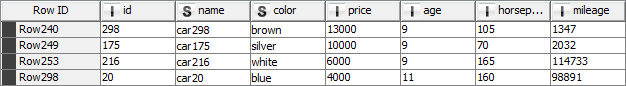
\includegraphics[width=0.6\textwidth]{domMaximizerOutput.png}
	\caption{Repräsentative Skyline des DominationMaximizer}
	\label{img:domMaximizerOutput}
\end{figure} 

Als nächstes wird der E-Greedy Node benutzt, um eine repräsentative Skyline zu bestimmen. Der Algorithmus beachtet sowohl Signifikanz als auch Diversität. Um signifikante Datensätze zu bestimmen, müssen die bereits existierenden Präferenzen mit weiteren Präferenzen erweitert werden. Für dieses Beispiel entscheidet der Kunde, dass er kein Auto mit einem höheren Preis als 16000 \euro haben möchte. Ergänzend sollte das Auto mehr als 100 PS besitzen. Somit wird für die Dimension price eingestellt, dass ein einzelner Threshold als obere Grenze berücksichtigt werden soll. Für die Dimension horsepower wird auch ein einzelner Threshold benutzt, jedoch als untere Grenze. Somit sind Datensätze signifikant, falls der Preis kleiner oder gleich 16000 \euro ist und die PS Leistung 100 oder mehr beträgt.
Für dieses Beispiel wird angenommen, dass Signifikanz wichtiger ist als Diversität. Aus diesem Grund wird der Diversitätsfaktor gleich $0.4$ gesetzt und dadurch der Signifikanzfaktor automatisch auf $0.6$. Für $k$ wird wieder ein Wert von vier genommen, da aus dieser kleinen Menge ein passendes Auto für den Kunden herausgesucht werden kann und nicht zu viele durch den Algorithmus wegfallen. Das Ergebnis dieses Algorithmus kann in Figur \ref{img:eGreedyOutput} betrachtet werden.

\begin{figure}[H]
	\centering
	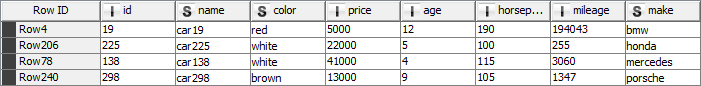
\includegraphics[width=0.6\textwidth]{eGreedyOutput.png}
	\caption{Repräsentative Skyline des E-Greedy}
	\label{img:eGreedyOutput}
\end{figure} 

Zum Schluss wird noch die Funktionsweise des DistanceBasedResolver Nodes vorgestellt. Da dieser Node nur die ersten zwei Dimensionen bei der Bestimmung der repräsentativen Skyline betrachtet, wurde ein neuer PreferenceCreator Node mit neuen Präferenzen erstellt. Es soll ein Auto gefunden werden mit einem niedrigen Preis und einer hohen PS Leistung (siehe Figur \ref{img:distanceNodeDialog}). Das Ergebnis des BlockNestedLoops sind vier Datensätze, welche durch den DistanceBasedResolver auf zwei runter reduziert werden sollen. Hierfür wurde im NodeDialog der entsprechende Parameter, um die Anzahl der ausgegebenen Datensätze zu reduzieren, auf zwei gesetzt. Das Ergebnis des Nodes ist in Abbildung \ref{distanceOutput} zu erkennen.

\begin{figure}[H]
	\centering
	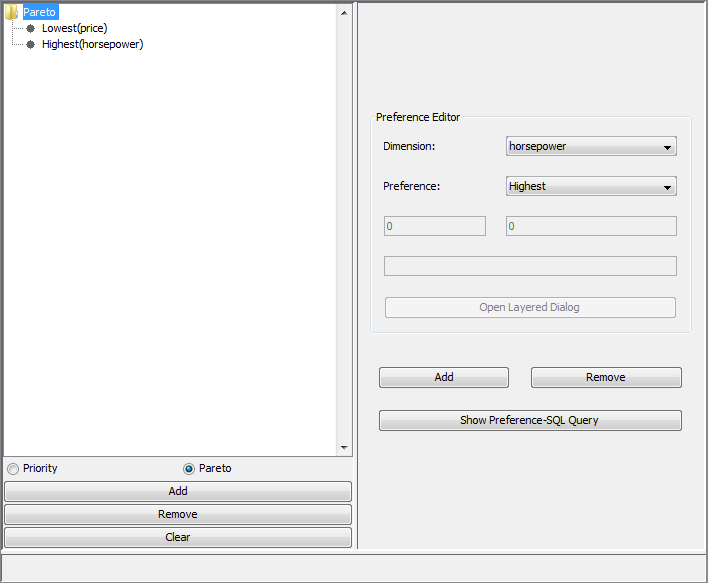
\includegraphics[width=0.6\textwidth]{distanceNodeDialog.png}
	\caption{NodeDialog des PreferenceCreator mit nur zwei Dimensionen}
	\label{img:distanceNodeDialog}
\end{figure} 

\begin{figure}[H]
	\centering
	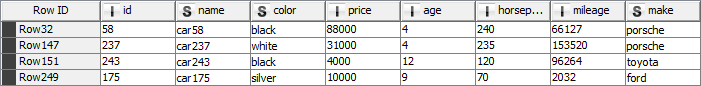
\includegraphics[width=0.6\textwidth]{distanceOutput.png}
	\caption{Repräsentative Skyline des DistanceBasedResolver}
	\label{img:distanceOutput}
\end{figure} 

Der aktuelle Workflow mit allen (repräsentativen) Skyline Nodes und dem zusätzlichen PreferenceCreator Node kann in Abbildung \ref{img:skylineWorkflow} gesehen werden.

\begin{figure}[H]
	\centering
	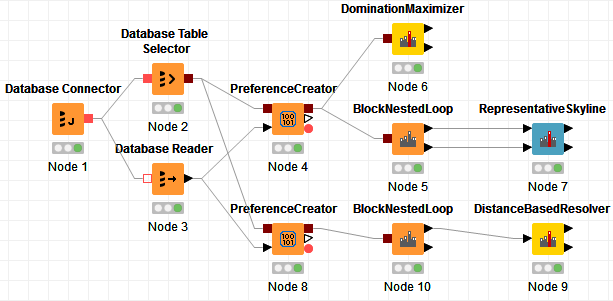
\includegraphics[width=0.6\textwidth]{skylineWorkflow.png}
	\caption{Workflow mit BlockNestedLoop, E-Greedy Node und DistanceBasedResolver Nodes}
	\label{img:skylineWorkflow}
\end{figure} 
%% ==============================
\section{Visualisierung}
\label{ch:Evaluierung:sec:visualize}
%% ==============================
Für die Visualisierung der Ausgaben der Nodes wird der SkylineVisualizer verwendet. Dieser nimmt als Eingabe zwei BufferedDataTables und erstellt mit diesen Daten ein Koordinatensystem mit dominierten und undominierten Punkten. Der erste BufferedDataTable sollte somit die undominierten und der zweite die dominierten oder alle Daten enthalten. Die Ausgaben des E-Greedy, DominationMaximizer und des DistanceBaseResolver Nodes sind jeweils zwei BufferedDataTable mit dominierten und undominierten Punkten und deswegen kann der SkylineVisualizer Node die Ausgaben dieser Nodes in einem Koordinatensystem darstellen.

Diese drei Nodes berechnen die repräsentative Skyline. Für eine repräsentative Skyline besteht das Koordinatensystem aus den repräsentativen Skylinepunkten als undominierte Punkte und den Skylinepunkten als dominierte Punkte. Falls drei Dimensionen betrachtet werden, erstellt der SkylineVisualizer für jede Kombination der Dimensionen einen Graph. Aus diesem Grund werden bei mehr als drei Dimensionen keine Graphen mehr erstellt. Dies bedeutet, dass keine Graphen für das ursprüngliche Beispiel erstellt werden können. Infolgedessen werden neue DominationMaximizer und EGreedy Nodes für das zwei dimensionale Beispiel erstellt. Die Eingabe bleiben bis auf dem Parameter $k$ identisch. Der Parameter $k$ wird auf zwei gesetzt, um die Skyline zu reduzieren und dadurch nicht alle Skylinedatensätze ausgegeben werden. 

Der Graph des DominationMaximizer Nodes kann in Abbildung \ref{img:domMaximizerView} gesehen werden. Wohingegen die Graphen des DistanceBaseResolver in Figur \ref{img:eGreedyView} und des E-Greedy in Figur \ref{img:distBasedResolverView} betrachtet werden können. 

\begin{figure}[H]
	\centering
	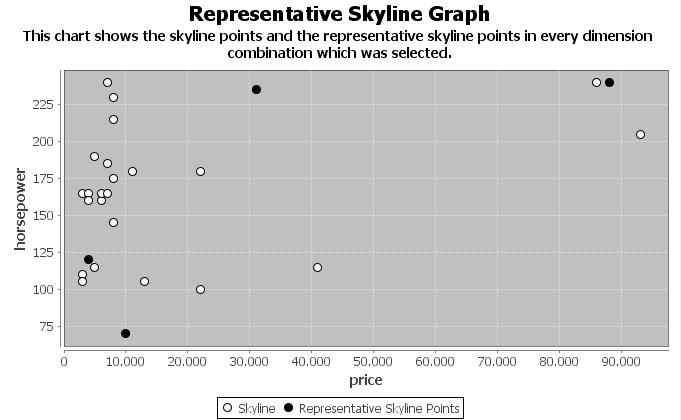
\includegraphics[width=0.6\textwidth]{domMaximizerView.png}
	\caption{SkylineVisualizer View für den DominationMaximizer Node}
	\label{img:domMaximizerView}
	
\end{figure} 
	\begin{figure}[H]
	\centering
	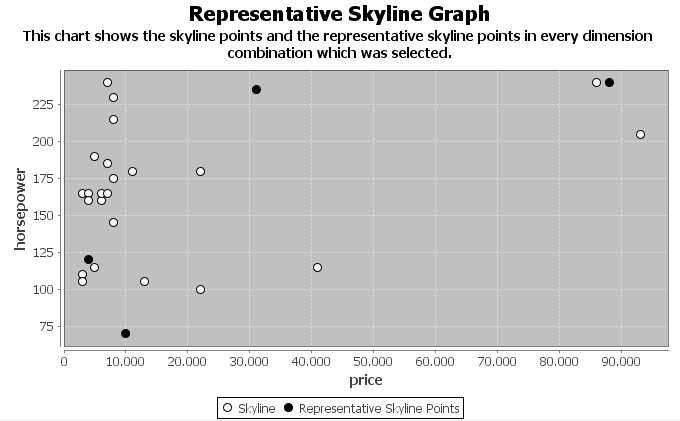
\includegraphics[width=0.6\textwidth]{eGreedyView.png}
	\caption{SkylineVisualizer View für den E-Greedy Node}
	\label{img:eGreedyView}
\end{figure} 

\begin{figure}[H]
	\centering
	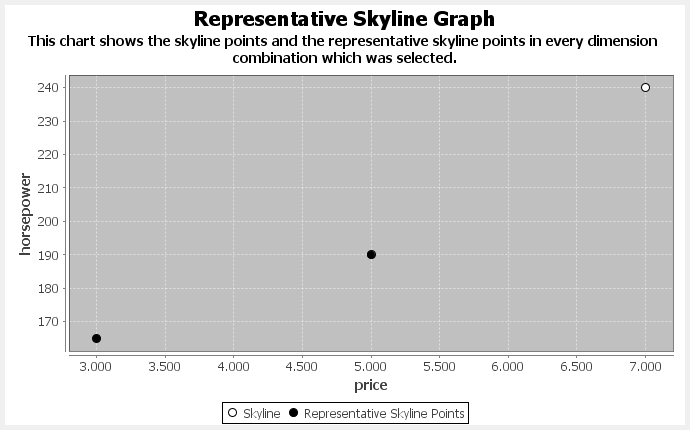
\includegraphics[width=0.6\textwidth]{distBasedResolverView.png}
	\caption{SkylineVisualizer View für den DistanceBasedResolver Node}
	\label{img:distBasedResolverView}
\end{figure} 

Der derzeitige Workflow mit den zusätzlichen SkylineVisualizer Nodes sieht dann wie in Abbildung \ref{img:visualizeWorkflow} aus.

\begin{figure}[H]
	\centering
	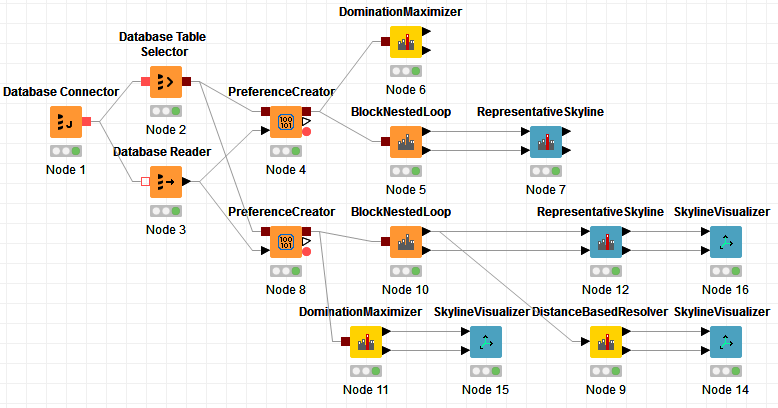
\includegraphics[width=0.6\textwidth]{visualizeWorkflow.png}
	\caption{Workflow mit dem Skyline Visualizer Node}
	\label{img:visualizeWorkflow}
\end{figure} 

%% ==============================
\section{Preference-SQL}
\label{ch:Evaluierung:sec:prefSQL}
%% ==============================
Zum Schluss werden nun noch der SQLExtractor und der PreferenceSQL Node zum Workflow hinzugefügt. Mithilfe des SQLExtractor Nodes kann der Preference-Query, der auf den erstellten Präferenzen basiert, betrachtet werden. Diesen Query benutzt der PreferenceSQL Node und fragt die Datenbank mit diesem Query ab. Dadurch werden die Best Matches (Skyline) für die erstellten Präferenzen ausgegeben. Der Query für das originale Beispiel lautet:
 
\begin{verbatim}
SELECT * 
FROM (SELECT * FROM car) AS T 
PREFERRING ((price LOWEST PRIOR TO age LOWEST) 
AND (horsepower HIGHEST 
PRIOR TO color LAYERED (('green', 'black'), OTHERS, ('red')))
AND mileage LOWEST)
\end{verbatim}

Wohingegen der Query für das zwei dimensionale Beispiel folgendermaßen aufgebaut ist:

\begin{verbatim}
SELECT * 
FROM (SELECT * FROM car) AS T 
PREFERRING (price LOWEST AND horsepower HIGHEST)
\end{verbatim}

Der schlussendliche Workflow ist in Abbildung \ref{img:finalWorkflow} zu sehen. 
 
\begin{figure}[H]
	\centering
	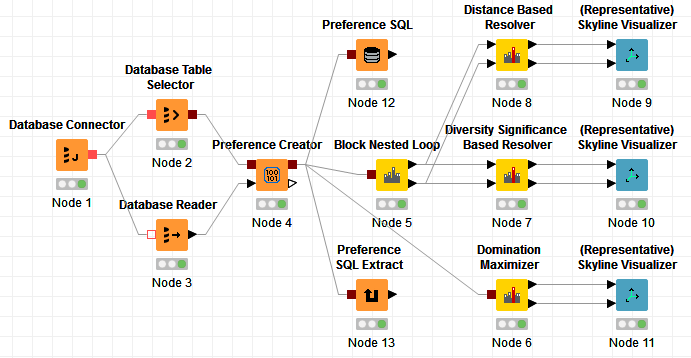
\includegraphics[width=0.6\textwidth]{finalWorkflow.png}
	\caption{Workflow mit PreferenceSQLExtractor und PreferenceSQL Node}
	\label{img:finalWorkflow}
\end{figure} 
%% ==============================
\section{Zusammenfassung}
\label{ch:Evaluierung:sec:zusammenfassung}
%% ==============================
Die Datensätze der repräsentativen Skyline können dem Kunden zum Schluss vorgezeigt werden. Woraufhin dieser sich für eines der Autos entscheiden kann. Es ist zu erkennen, dass der Kunde mit vier Autos eine übersichtlichere Menge für die Entscheidung hat als bei 27 vorliegenden Datensätzen.

Zusammenfassend kann gesagt werden, dass die KNIME Nodes intuitiv und einfach nutzbar sind. Durch die Auswahl und Eingrenzen der Kriterien mithilfe der Nodes konnten schnell die besten Auto für die Präferenzen des Kunden gefunden werden. Visualisierungen helfen dabei die repräsentativen Datensätze einordnen zu können. 
%% ==============================
%%% End: 